\section{Results}\label{sec:results}

We organize the evidence around the three hypotheses, after first confirming that our measurement pipeline reproduces known facts about the base-to-instruct shift. All numbers are computed on \justeval{} response tokens, with the predictor trained on the disjoint \dolly{} corpus.

\subsection{Measurement validation}

\para{We reproduce URIAL's stylized facts.} Before reading residuals, we check that teacher-forcing both models under the identical chat-formatted context recovers the qualitative picture established by \citet{lin2023urial}. Across the three \qwen{} pairs, the base and instruct models agree on the top-1 next token at \textbf{83--85\%} of response positions, closely matching URIAL's $\sim$78\% (their estimate is on a different family and decoding setup, so near-agreement is the expected outcome). The mean per-token \klt{} is small, \textbf{0.21--0.24 nats}, confirming that most of the response is generated by tokens on which the two models barely disagree. This is the backdrop against which a learned predictor has any hope of working: the shift is concentrated, not uniform.

\para{The shift is front-loaded.} \Figref{fig:kl_vs_pos} shows that divergence is sharply position-dependent. For \qwensmall{}, mean \klt{} falls from \textbf{0.68 nats at positions 0--4 to 0.12 nats at positions 40+}, a roughly $6\times$ decay. Instruction tuning rewrites the opening of a response---where the model commits to a stance, a format, or a refusal---and then largely defers to the base distribution once the response is underway. {\bf Is position therefore the story?} We show next that it is not: position alone explains almost none of the variance once we condition on what the base model was already doing.

\begin{figure}[t]
    \centering
    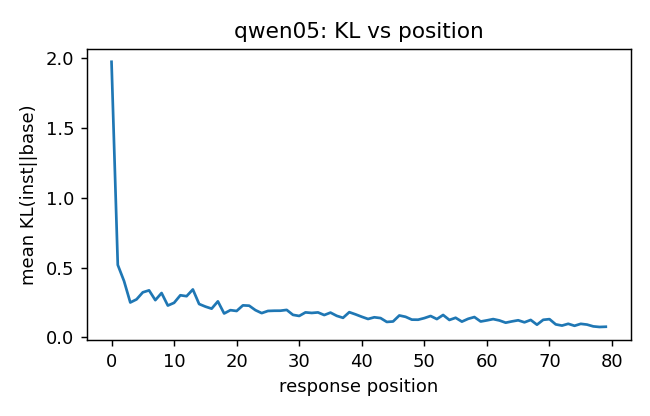
\includegraphics[width=0.6\linewidth]{figures/qwen05_kl_vs_pos.png}
    \caption{Mean per-token \klt{} as a function of response position for \qwensmall{}. Divergence is strongly front-loaded, decaying from $\sim$0.68 nats in the first few tokens to $\sim$0.12 nats after position 40. Instruction tuning chiefly rewrites the start of a response. Shaded band shows the standard error within each position bin.}
    \label{fig:kl_vs_pos}
\end{figure}

\subsection{H1: per-token KL is largely predictable}

\para{A simple base-side predictor captures most of the divergence.} We train the \gbt{} on \dolly{} and evaluate on \justeval{}, so any signal it captures is cross-corpus and cannot be leakage. \Tabref{tab:predictability} reports the result: cross-corpus $R^2$ is \textbf{0.599} (\qwensmall), \textbf{0.680} (\qwenmid), and \textbf{0.626} (\qwenbig), with validation $R^2$ in the same 0.62--0.70 range. Rank agreement is even stronger---Spearman $\rho(\text{pred},\text{actual})$ reaches \textbf{0.82 / 0.85 / 0.89} as we scale. Two-thirds of the per-token variance in \klt{} is anticipated from features that never look at the instruct model.

\begin{table}[t]
    \centering
    \resizebox{\textwidth}{!}{%
    \begin{tabular}{@{}lcccccccc@{}}
        \toprule
        \multirow{2}{*}{\textbf{Pair}} & \multirow{2}{*}{\textbf{top-1 agree}} & \multirow{2}{*}{\textbf{mean KL}} & \multicolumn{3}{c}{\textbf{Baseline} $R^2$ \textbf{(val)}} & \multicolumn{2}{c}{\textbf{\gbt} $R^2$} & \multirow{2}{*}{\textbf{Spearman} $\rho$} \\
        \cmidrule(lr){4-6} \cmidrule(lr){7-8}
        & & & pos-only & entropy-only & base-logp-only & val & x-corpus & \\
        \midrule
        \qwensmall & 0.829 & 0.207 & 0.015 & 0.196 & 0.398 & \textbf{0.704} & \textbf{0.599} & 0.821 \\
        \qwenmid   & 0.852 & 0.214 & 0.046 & 0.394 & 0.382 & \textbf{0.693} & \textbf{0.680} & 0.849 \\
        \qwenbig   & 0.826 & 0.240 & 0.022 & 0.281 & 0.510 & \textbf{0.621} & \textbf{0.626} & 0.885 \\
        \bottomrule
    \end{tabular}
    }
    \caption{\textbf{Per-token KL is largely predictable from base-side context, and position alone is nearly useless.}
    Top-1 agreement and mean per-token $\klt$ (nats) measured on \justeval. Predictor $R^2$ on a held-out validation
    split of \dolly\ (val) and on the disjoint \justeval\ corpus (x-corpus). The gradient-boosted predictor (\gbt)
    explains $\sim$60--68\% of cross-corpus KL variance, far above every single-feature baseline; position-only
    regression is near-zero ($R^2 \le 0.05$). Spearman $\rho$ is between predicted and actual KL on \justeval.
    Best per-row \gbt\ values in \textbf{bold}.}
    \label{tab:predictability}
\end{table}


\para{The signal is base entropy and base surprise, not position or token type.} \Figref{fig:featimp} and \Tabref{tab:featimp} make the source of the predictability explicit. The base model's log-probability of the emitted token (\texttt{base\_tok\_logprob}) and its predictive entropy (\texttt{base\_entropy}) dominate, with importances of \textbf{$\sim$0.4--0.6 each}; position contributes only $\sim$0.03--0.08, and every stylistic, lexical, and token-class flag sits below 0.03. Single-feature baselines confirm the ranking: a position-only model is near useless ($R^2$ \textbf{0.015--0.046}), an entropy-only model reaches 0.196/0.394/0.281, and a base-logprob-only model reaches 0.398/0.382/0.510. {\bf What does this refine?} URIAL frames the shift as decaying with position; we find that decay is \emph{entropy-mediated}. Early tokens diverge because the base model is uncertain there; once the base distribution sharpens, instruction tuning has little room to move it. Position is a proxy for surprise, not a cause.

\begin{table}[t]
    \centering
    \resizebox{0.7\textwidth}{!}{%
    \begin{tabular}{@{}lccc@{}}
        \toprule
        \textbf{Feature} & \qwensmall & \qwenmid & \qwenbig \\
        \midrule
        \texttt{base\_tok\_logprob} & \textbf{0.603} & 0.399 & \textbf{0.609} \\
        \texttt{base\_entropy}      & 0.496 & \textbf{0.657} & 0.139 \\
        \texttt{base\_top1\_prob}   & 0.273 & 0.139 & 0.427 \\
        \texttt{pos}                & 0.076 & 0.077 & 0.033 \\
        \texttt{tok\_len}           & 0.012 & 0.016 & 0.017 \\
        \texttt{is\_punct}          & 0.011 & 0.002 & 0.026 \\
        \texttt{is\_stylistic}      & 0.010 & 0.015 & 0.003 \\
        \texttt{is\_wordlead}       & 0.004 & 0.015 & 0.006 \\
        \texttt{is\_number}         & 0.001 & 0.000 & 0.001 \\
        \bottomrule
    \end{tabular}
    }
    \caption{\textbf{Predictive structure is base-model uncertainty, not position or lexical class.}
    Gradient-boosting feature importance (gain) for the \gbt\ divergence predictor across all three pairs.
    Base token surprise (\texttt{base\_tok\_logprob}) and base entropy (\texttt{base\_entropy}) dominate;
    response position (\texttt{pos}) and every stylistic/lexical flag contribute little. This refines URIAL's
    ``KL decays with position'': the decay is mostly \emph{mediated by entropy decay}, not position per se.
    Largest per-column value in \textbf{bold}.}
    \label{tab:featimp}
\end{table}


\begin{figure}[t]
    \centering
    \begin{subfigure}{0.32\textwidth}
        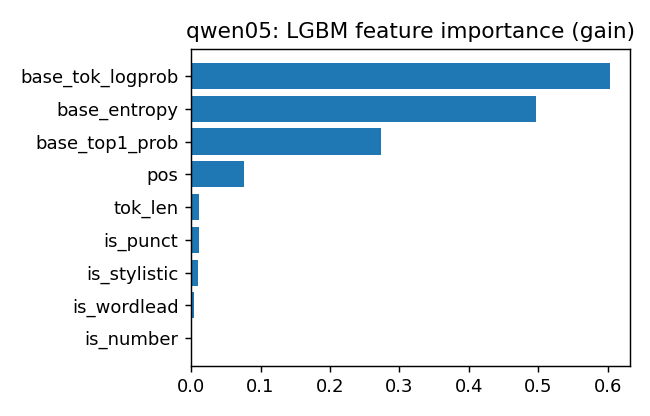
\includegraphics[width=\linewidth]{figures/qwen05_featimp.png}
        \caption{\qwensmall{}}
    \end{subfigure}
    \hfill
    \begin{subfigure}{0.32\textwidth}
        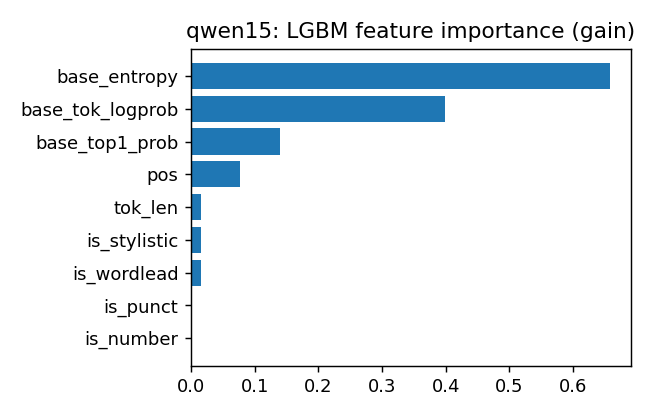
\includegraphics[width=\linewidth]{figures/qwen15_featimp.png}
        \caption{\qwenmid{}}
    \end{subfigure}
    \hfill
    \begin{subfigure}{0.32\textwidth}
        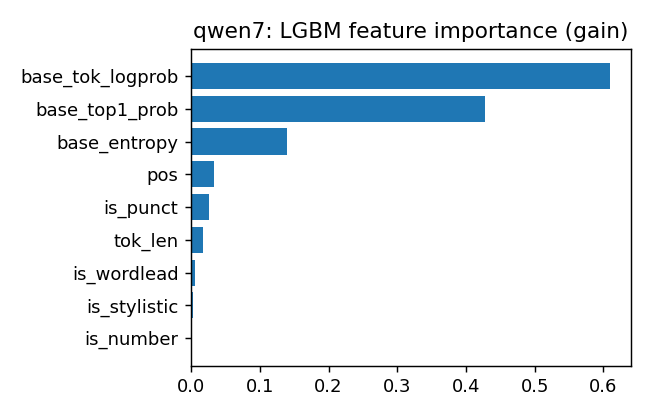
\includegraphics[width=\linewidth]{figures/qwen7_featimp.png}
        \caption{\qwenbig{}}
    \end{subfigure}
    \caption{\gbt{} feature importances for predicting per-token \klt{}, across all three model pairs. Two base-side quantities---the base log-probability of the emitted token and the base predictive entropy---dominate, while position and all stylistic, lexical, and token-class flags are negligible ($<$0.03). The predictable component of the base-to-instruct shift is governed by where the base model is already uncertain.}
    \label{fig:featimp}
\end{figure}

\para{The predictor is well-calibrated.} \Figref{fig:calibration} shows predicted versus actual \klt{} for \qwensmall{}; points track the diagonal across the bulk of the range, so the residuals we analyze next are genuine prediction errors rather than systematic miscalibration. This is what licenses reading residuals as ``surprises.''

\begin{figure}[t]
    \centering
    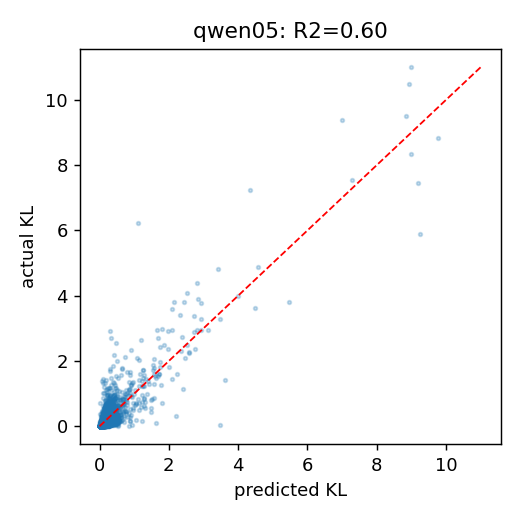
\includegraphics[width=0.55\linewidth]{figures/qwen05_calibration.png}
    \caption{Predicted versus actual per-token \klt{} on held-out \justeval{} tokens for \qwensmall{}. Predictions track the diagonal across the bulk of the range, confirming the \gbt{} is calibrated rather than merely correlated, so the residual (actual $-$ predicted) is a clean signal of what the base-side features fail to anticipate.}
    \label{fig:calibration}
\end{figure}

\subsection{H2: the residual is structured}

\para{The leftover variance is not noise.} If the residual were homogeneous prediction error, it would be unrelated to token identity. It is not. A Kruskal--Wallis test across token classes rejects equality of residual distributions at \textbf{$p<10^{-22}$ for every pair} (\qwensmall{} $2.9\times10^{-29}$, \qwenmid{} $1.2\times10^{-23}$, \qwenbig{} $1.3\times10^{-88}$). The residual also varies systematically across position bins even though position is itself an input feature the \gbt{} could already exploit---meaning the structure that remains is not capturable by position alone. The model has learned the smooth, entropy-driven backbone of the shift and left behind something organized that those features cannot reach.

\subsection{H3: the residual is alignment-specific}

\para{Safety prompts are systematically under-predicted.} The structure in the residual is exactly the content one would attribute to alignment, not to generic style. \Tabref{tab:safety_residual} compares the 200 safety-tagged \justeval{} instructions against the rest. Safety tokens carry a positive mean residual while regular tokens carry a near-zero or slightly negative one: \textbf{+0.138 vs $-$0.012} (\qwensmall{}, rank-biserial 0.322), \textbf{+0.085 vs $-$0.015} (\qwenmid{}, 0.302), and \textbf{+0.061 vs $-$0.012} (\qwenbig{}, 0.141). One-sided Mann--Whitney tests are overwhelming ($p\approx0$ for \qwensmall{}, $3\times10^{-284}$ for \qwenmid{}, $2\times10^{-164}$ for \qwenbig{}). The predictor consistently \emph{underestimates} divergence on safety content: the instruct model moves more than its base-side surprise would imply. The effect shrinks with scale---larger base models already place more mass on safety-consistent continuations---but remains highly significant everywhere.

\begin{table}[t]
    \centering
    \resizebox{0.85\textwidth}{!}{%
    \begin{tabular}{@{}lccccc@{}}
        \toprule
        \textbf{Pair} & \textbf{mean resid (safety)} & \textbf{mean resid (regular)} & \textbf{rank-biserial} & \textbf{$p$} \\
        \midrule
        \qwensmall & \textbf{+0.138} & $-0.012$ & 0.322 & $\approx 0$ \\
        \qwenmid   & \textbf{+0.085} & $-0.015$ & 0.302 & $3\!\times\!10^{-284}$ \\
        \qwenbig   & \textbf{+0.061} & $-0.012$ & 0.141 & $2\!\times\!10^{-164}$ \\
        \bottomrule
    \end{tabular}
    }
    \caption{\textbf{The residual concentrates on safety prompts in every pair.}
    Mean prediction residual ($\text{actual KL} - \text{predicted KL}$) on safety vs.\ regular \justeval\ prompts,
    with one-sided Mann--Whitney $p$ and rank-biserial effect size. Safety prompts are exactly where the predictor
    most \emph{under}-estimates divergence. The effect shrinks with scale (0.322 $\to$ 0.302 $\to$ 0.141) but
    remains overwhelmingly significant. Larger safety mean residual in \textbf{bold}.}
    \label{tab:safety_residual}
\end{table}


\para{Two interpretable token families drive the residual.} \Tabref{tab:residual_tokens} lists the highest-residual token strings. They fall into two recognizable groups. The first is \emph{discourse and structural pivots}: tokens like \emph{Additionally}, \emph{However}, \emph{Instead}, \emph{Specifically}, \emph{Such}, and---most tellingly---refusal-recovery openers. In a concrete \qwensmall{} case, after declining a request the instruct model emits ``\emph{If} you have any other questions\ldots''; the base model ranks \emph{If} only third at that position, and the per-token \klt{} spikes to \textbf{$\sim$19.9 nats}. This is a learned move---softening a refusal by re-offering help---that the base distribution gives no hint of. The second group is \emph{safety, persona, identity, and helpfulness injections}: \emph{Safety}, \emph{guidelines}, \emph{violence}, \emph{politics}, \emph{discuss}, \emph{provide}, \emph{recommend}, alongside \emph{assistant} and \emph{Alibaba} (Qwen's maker, an identity injection) and \emph{October} (knowledge-cutoff framing). \Figref{fig:resid_category} aggregates these into per-category residual distributions, and \Figref{fig:summary} shows the picture is consistent across all three pairs: high predictability of the bulk shift, a structured residual, and that residual concentrated on alignment-specific tokens. Crucially, the stylistic tokens that dominate the \emph{predictable} shift (punctuation, function words, formatting) do \emph{not} appear here---the surprise is alignment, not style.

\begin{table}[t]
    \centering
    \resizebox{\textwidth}{!}{%
    \begin{tabular}{@{}llp{10.5cm}@{}}
        \toprule
        \textbf{Pair} & \textbf{Family} & \textbf{Highest-residual token strings} (mean residual, $n\!\ge\!5$) \\
        \midrule
        \multirow{2}{*}{\qwensmall}
          & Discourse pivots & \texttt{Additionally}, \texttt{If}, \texttt{However}, \texttt{The}, \texttt{Building}, \texttt{Subject} \\
          & Safety / sensitive & \texttt{politics}, \texttt{sex}, \texttt{violence}, \texttt{encourage}, \texttt{distress}, \texttt{sensitive}, \texttt{political} \\
        \midrule
        \multirow{2}{*}{\qwenbig}
          & Discourse pivots & \texttt{If}, \texttt{Such}, \texttt{However}, \texttt{Instead}, \texttt{Specifically}, \texttt{For} \\
          & Safety / persona / helpfulness & \texttt{Safety}, \texttt{guidelines}, \texttt{assistant}, \texttt{Alibaba}, \texttt{October}, \texttt{provide}, \texttt{recommend}, \texttt{discuss} \\
        \bottomrule
    \end{tabular}
    }
    \caption{\textbf{The unpredictable residual recovers exactly what alignment installs.}
    Token strings with the highest mean residual on \justeval, grouped into two interpretable families: (i)
    discourse/structural pivots at clause boundaries (\eg refusal-recovery openers such as \texttt{If}), and (ii)
    safety/persona/identity/helpfulness injections (\eg \texttt{Safety}, \texttt{guidelines}, \texttt{Alibaba} ---
    Qwen's maker, an identity injection). Neither family is the generic stylistic token (\texttt{Here}, \texttt{However})
    that the predictor already accounts for.}
    \label{tab:residual_tokens}
\end{table}


\begin{figure}[t]
    \centering
    \begin{subfigure}{0.32\textwidth}
        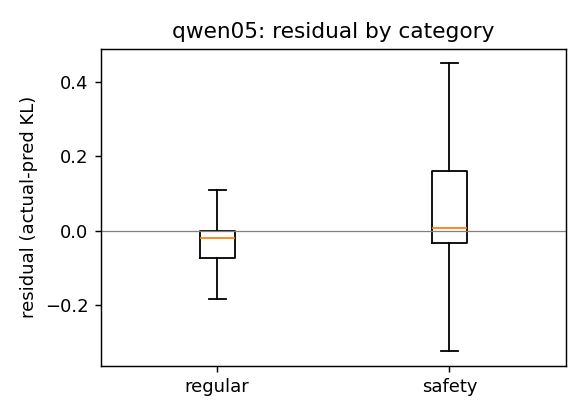
\includegraphics[width=\linewidth]{figures/qwen05_resid_category.png}
        \caption{\qwensmall{}}
    \end{subfigure}
    \hfill
    \begin{subfigure}{0.32\textwidth}
        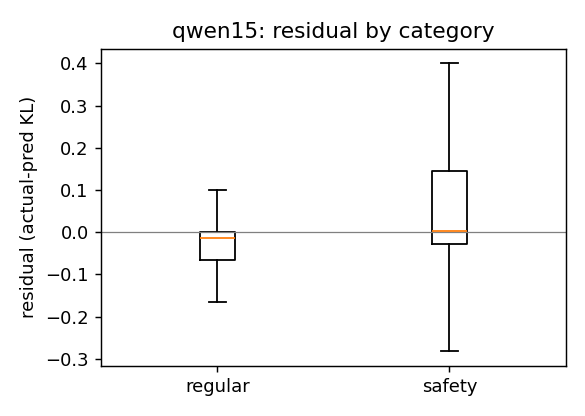
\includegraphics[width=\linewidth]{figures/qwen15_resid_category.png}
        \caption{\qwenmid{}}
    \end{subfigure}
    \hfill
    \begin{subfigure}{0.32\textwidth}
        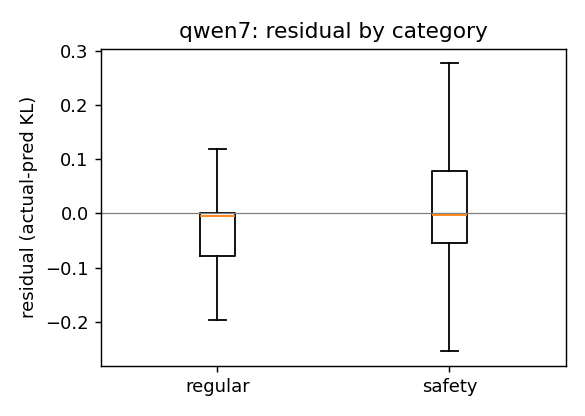
\includegraphics[width=\linewidth]{figures/qwen7_resid_category.png}
        \caption{\qwenbig{}}
    \end{subfigure}
    \caption{Mean residual (actual $-$ predicted \klt{}) by token category, across all three model pairs. Safety, discourse-pivot, and persona/identity categories sit well above zero, while generic stylistic and lexical categories sit at or below it. The base-side predictor systematically under-predicts exactly the alignment-relevant tokens.}
    \label{fig:resid_category}
\end{figure}

\begin{figure}[t]
    \centering
    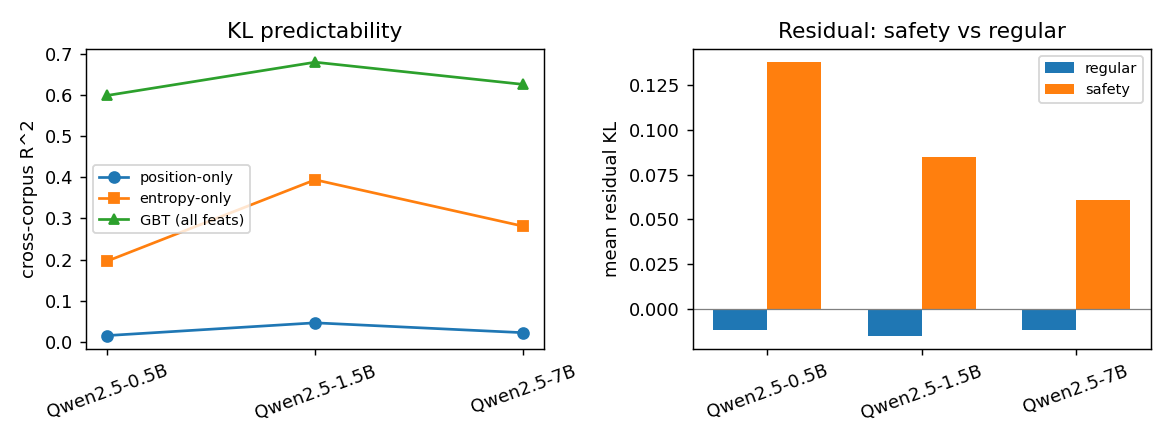
\includegraphics[width=0.9\linewidth]{figures/summary_across_pairs.png}
    \caption{Summary across the three \qwen{} pairs (\qwensmall{}, \qwenmid{}, \qwenbig{}). Left to right: cross-corpus predictor $R^2$ (0.60--0.68), the safety-vs-regular residual gap (positive and significant in every pair, shrinking with scale), and the dominance of base entropy and base token surprise in feature importance. The bulk base-to-instruct shift is predictable from base-side context; what is left over is structured and alignment-specific.}
    \label{fig:summary}
\end{figure}
